% !TEX root = Thesis.tex

%==============================================================================
\chapter{Erbium \acl*{bec}}
\label{chap:erbium_bec}
%==============================================================================

This chapter has the objective of briefly review some relevant properties of Erbium, which will clarify what makes it relevant in the study of ultra cold atoms. After this, the basic theory of Bose-Einstein condensation will be discussed, along with a brief description of the experimental phases and tools required to create and observe an Erbium \ac{bec}. This experimental realization will be the foundation on which the following chapters will be grounded when discussing further experimental achievements.

%==============================================================================
\section{Properties of erbium} \label{sec:erbium_properties}
%==============================================================================
Erbium is a chemical element with an atomic number of 68, which belongs to the series of the Lanthanides. It is also part of the group called Rare-earth elements and it was first discovered by G. Monsander in 1843 \cite{mosander1843xxx}. The name of ``Erbium'' comes from the name of the Swedish village of Ytterby, the place where it was extracted. At that time, the similarity of rare-earth metals' chemical properties made their distinction extremely difficult. For this reason, what G. Monsander thought to be pure Erbium oxide was in fact a mixture of different rare-earth metal oxides. The element is not obtained in a reasonably pure form until 1937 by W. Klemm and H. Bommer \cite{klemm1937bommer}.

Considering some basic properties of this element, under standard conditions erbium is in a solid state. It has a silver shining surface, which oxidizes with air contact. This rare-earth metal has a melting point of \SI{1802}{\kelvin} and boiling point of \SI{3136}{\kelvin}. As a result, to be able to work with a free atomic gas of erbium requires to heap up the solid erbium metal to high temperatures \cite{emsley1998}.

The number of stables isotopes of Erbium is 6 and they can be seen in Table \ref{tab:Isotopes_Erbium}. All of them are bosons with nuclear spin of zero, in exception of $^{\text{167}}\text{Er}$, which is a fermion with spin of 7/2. The chosen isotope for this experiment is $^{\text{168}}\text{Er}$ because of its bosonic nature (see Section \ref{sec:bose-einstein_condensation}), high abundance and favorable scattering properties.

\begin{table}[htbp] \centering
	\begin{tabular}{@{}c|c|c|c@{}}\hline
		Isotope                  & Abundance [\%]          & Atomic Mass [u] & Nuclear Spin [$\hbar$] \\ \hline\hline
		$\text{Er}^{\text{162}}$ &  0.14                   & 161.928775      & 0   \\
		$\text{Er}^{\text{164}}$ &  1.61                   & 163.929198      & 0   \\ 
		$\text{Er}^{\text{166}}$ & 33.60                   & 165.930290      & 0   \\
		$\text{Er}^{\text{167}}$ & 22.95                   & 166.932046      & 7/2   \\
		$\text{Er}^{\text{168}}$ & 26.80                   & 167.932368      & 0   \\  
		$\text{Er}^{\text{170}}$ & 14.90                   & 169.935461      & 0   \\  \hline
	\end{tabular}
	\caption[Table with the stable isotopes of Erbium]{Table with the stable isotopes of Erbium that can be found on Nature with their respective Abundance ratio, Atomic mass and Nuclear Spin. Spectroscopy data taken from \cite{sansonetti2005handbook}.}\label{tab:Isotopes_Erbium}
\end{table}

In addition to these properties, erbium atoms have a rather complex energetic level scheme due to its open 4f shell. This one lacks 2 electrons to be completely filled, which makes erbium to have an electronic ground state with an orbital angular momentum value of $L = 5$ and a high magnetic moment of seven Bohr magneton $7\mu_B$ \cite{ban2005laser}. This high value for the orbital angular momentum in the ground state of erbium provides several advantages for Raman-coupling processes. Leading to longer coherence times and stronger synthetic magnetic fields when comparing with other alkali metals like rubidium or cesium, commonly used in ultracold atoms experiments  \cite{cui2013synthetic}.


A scheme of erbium energy levels together with the atomic transitions used in this experiment can be seen in figure \ref{fig:erbium_scheme}. The scheme shows that the electronic ground state of erbium is $\text{[Xe] }\text{4f}^{12} \text{6s}^2$, where [Xe]
represents the complete electronic configuration of Xenon\footnote{$\text{[Xe] = }\text{1s}^2 \text{ 2s}^2 \text{ 2p}^6 \text{ 3s}^2 \text{ 3p}^6 \text{ 3d}^{10} \text{ 4s}^2 \text{ 4p}^6 \text{ 4d}^{10} \text{ 5s}^2 \text{ 5p}^6$}. Moreover, the used optical transitions are represented by colored arrows in the figure and its spectroscopic data is shown in table \ref{tab:Transitions}. From now on, these three transitions will respectively be referred to as the 401nm, 583nm, and 841nm transitions.

Finally, it must be noted that aside from the discussed application in ultracold atoms, erbium is used in multiple commercial applications. One prominent example is the use or erbium as a fiber amplifier in doped silicon fibers \cite{mears1987low}. Furthermore, in nuclear physics it is used as neutron absorbing control rods \cite{emsley2011nature}.

%\sisetup{per-mode = symbol}%

\begin{table}[htbp] \centering
	\begin{tabular}{@{}l|c|c|S|S|S@{}}\hline
		\multicolumn{3}{c|}{Parameters} & \multicolumn{3}{c}{Transitions} \\ \hline
		Name & Symbol & Unit & \multicolumn{1}{c|}{401nm} & \multicolumn{1}{c|}{583nm} & \multicolumn{1}{c}{841nm} \\ \hline\hline
		Wavelength in vacuum & $\lambda$	& \si{\nano\meter}					& 400.91		& 582.84		& 841.22\\
		Lifetime 			& $\tau$	& \si{\micro\second}				& 0.045			& 0.857			& 20   \\ 
		Natural linewidth 	& $\Delta \nu_0$	& \si{\kilo\hertz}					& \num{33370} 	& 185.71 		& 7.96   \\
		Decay rate 			& $\gamma$	& \si{\per\second}					& \num{2.22e8} 	& \num{1.17e6}  & \num{5.00e4} \\
		Saturation intensity & $I_{S}$	& \si{\milli\watt\per\centi\meter}	& 71.80			& 0.12			& 1.74  \\  
		Doppler temperature	& $T_D$	& \si{\micro\kelvin} 				& 848.69  		& 4.46  		& 0.19    \\  
		Doppler velocity	& $v_D$	& \si{\centi\meter\per\second}		& 21.5 			& 1.49 			& 0.31 \\
		Recoil temperature	& $T_R$	& \si{\nano\kelvin} 				& 354.95  		& 167.94  		& 80.43    \\  
		Recoil velocity	& $v_R$	& \si{\milli\meter\per\second}		& 5.93 			& 4.08 			& 2.82 \\  \hline
	\end{tabular}
	\caption[Spectroscopic data for the optical transitions of Erbium]{Spectroscopic data for the optical transitions of Erbium used in this experiment. These transitions are called the 401nm, 583nm, and 841nm transitions and can be seen in figure \ref{fig:erbium_scheme}. Shown spectroscopic data taken from \cite{mcclelland2006natural, lawler2010atomic, den2010radiative, ban2005laser, lipert1993isotope}}\label{tab:Transitions}
\end{table}


\pagebreak


\begin{figure}[!htbp]\centering
	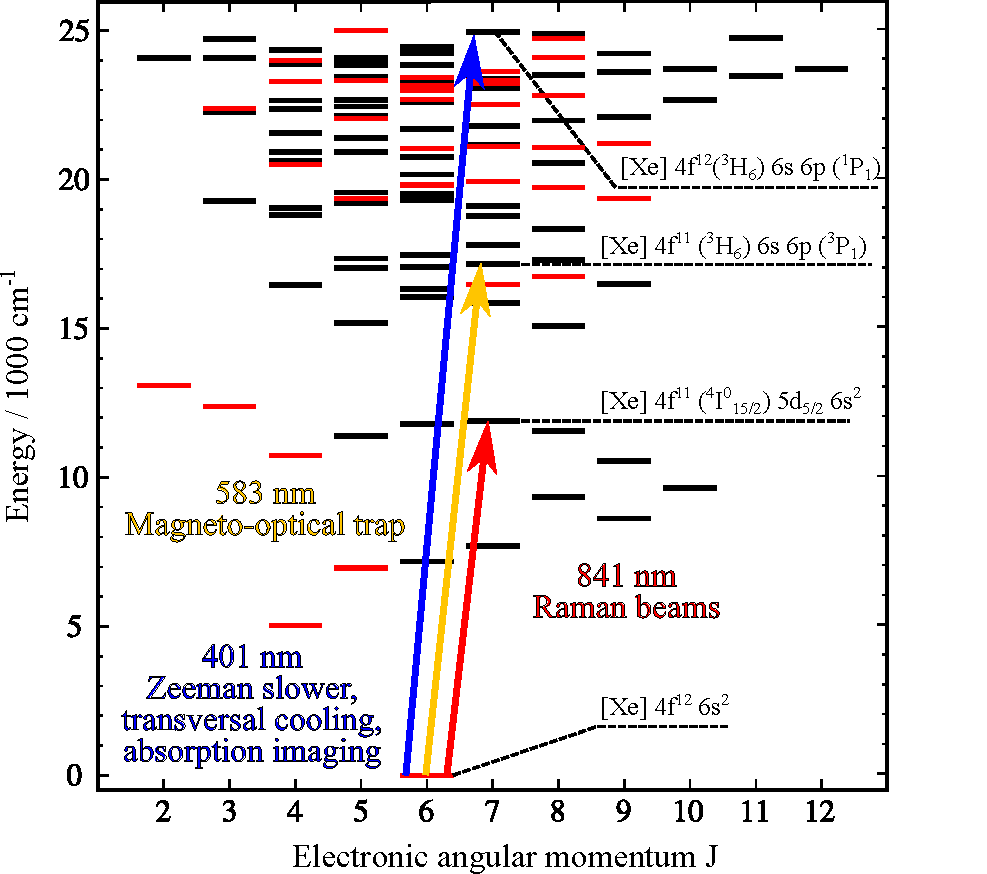
\includegraphics[width=1.\columnwidth]{erbium_term_scheme.pdf}
	\caption[Erbium energy scheme]{Energy level scheme of Erbium represented as a function of the total angular momentum J. This scheme shows only a range of energies relevant for the experiment of up to 25000 $\text{cm}^{\text{-1}}$. The different arrows show us the used transitions and for which phase of the experiment they are used for. The red lines represent energy states with even parity and the black lines those with odd parity. Data taken from \cite{NIST}. }\label{fig:erbium_scheme}
\end{figure}


%==============================================================================
\section{Bose-Einstein Condensation} \label{sec:bose-einstein_condensation}
%==============================================================================

A \ac{bec} is generally defined as a state of matter formed when a gas of bosons with a low density is cooled to near-zero temperatures (typically a few hundreds nanokelvins). To understand this definition and the next theoretical principles is necessary to define what is a Boson. In quantum mechanics, bosons are particles with an integer value in their spin. Because of this,  also have a symmetric wave function under the interchange of two particles, which allows bosons to have the same quantum state. Unlike its counterpart fermions, which have a half odd integer spin and an anti-symmetric wave function. Leading to Pauli's exclusion principle that avoids more than one fermion to occupy the same quantum state \cite{Pauli1925}.

It was the Indian physicist S. N. Bose in 1924, the first one who described in a successful way an ideal gas of non interacting free photons, behaving like mass-less bosons. His idea was initially rejected for publication in scientific journals. However, Bose sent the manuscript to A. Einstein, who recognized its importance, translated the paper to german and saw to it that was published \cite{Bose1924}. After this, Einstein extended Bose's treatment to massive particles and predicted the occurrence of a phase transition in a gas of non-interacting atoms, what is today known as a \ac{bec} \cite{Einstein1924, Einstein1925}.

These publications led to Bose-Einstein statistics, a model that explains the energetic behavior of a non-interacting gas of indistinguishable $N$ bosons, each one with mass $M$. The average number of particles at a given non-degenerate state with wave vector $\mathbf{k}$ and energy $E_\mathbf{k} = \hbar^2 \mathbf{k}^2 / 2M$ is given by

\begin{equation}\label{eq:bose-einstein_distribution}
	\bar{N}_{\mathbf{k}} = \frac{1}{e^{(E_\mathbf{k} - \mu)/k_B T} - 1}
\end{equation}
For an ideal gas of bosons in thermal equilibrium at a temperature $T$, Boltzmann constant $k_B$ and chemical potential $\mu$, which depends of $N$ and $T$ \cite{Masahito2010}. This relation can be expressed as

\begin{equation}\label{eq:chemical_potential_relation}
N = \sum_{\mathbf{k}}\frac{1}{e^{(E_\mathbf{k} - \mu)/k_B T} - 1}
\end{equation}

So the chemical potential $\mu$ is determined such that Eq. \eqref{eq:chemical_potential_relation} is satisfied for any given $N$ remaining constant. Now, expanding into the thermodynamic limit where $N$ and the occupied volume $V$ are increased to infinite values keeping the particle density $n = V/N$ constant. The sum over $\mathbf{k}$ appearing in Eq. \eqref{eq:chemical_potential_relation} can be replaced by an integral such as

\begin{equation}\label{eq:thermodynamic_limit}
n = \frac{N}{V} =  \frac{1}{(2\pi)^3}\int d^3 k\frac{1}{e^{(E_\mathbf{k} - \mu)/k_B T} - 1}
\end{equation}

For decreasing values of $T$ and constant $n$, the chemical potential increases becoming zero at a critical temperature $T_C$. By making $\mu = 0$, $T = T_C$ and $E_\mathbf{k} = \hbar^2 \mathbf{k}^2 / 2M$ in Eq. \eqref{eq:thermodynamic_limit} results

\begin{equation}\label{eq:thermodynamic_limit_at_critical_conditions}
n =  \zeta(3/2) \bigg(\frac{M k_B T_C}{2 \pi \hbar^2}\bigg)^{3/2}
\end{equation}
Where $\zeta(3/2) \simeq 2.612$ denotes the Riemann zeta function evaluated at 3/2. So the critical temperature of the \ac{bec} is given by

\begin{equation}\label{eq:critical_temperature}
T_C = 3.31 \frac{\hbar^2 n^{2/3}}{k_B M}
\end{equation}

A relevant case of study is when $T < T_C$ because a fraction of the $N$ bosons remains in the ground state with an energy $E = 0$. So the ideal gas of bosons can be divided in two energetic groups $N = N_{E=0} + N_{E>0}$. It must be noted that, the replacement of a sum by an integral in Eq. \eqref{eq:thermodynamic_limit} can only be take place in group of particles with an energy greater than zero $E>0$. As a result of this, the integral of Eq. \eqref{eq:thermodynamic_limit} for the case $T < T_C$ results

\begin{equation}\label{eq:thermodynamic_limit_low_T}
\frac{N_{E>0}}{V} = \zeta(3/2) \bigg(\frac{M k_B T}{2 \pi \hbar^2}\bigg)^{3/2}
\end{equation}

Using now equations \eqref{eq:critical_temperature}, \eqref{eq:thermodynamic_limit_at_critical_conditions} and the fact that $N_{E>0} = N - N_{E=0}$ results in an expression of the relative population of a \ac{bec} in an ideal bosons gas as a function of temperature:

\begin{equation}\label{eq:bec_relative_population}
\frac{N_{E=0}}{N} = 1 - \bigg(\frac{T}{T_C}\bigg)^{3/2}
\end{equation}

An intuitive way to think about this is to imagine the bosons as wave packets with a size of the thermal de Broglie length $\lambda_{th}$. This parameter is conventionally defined \cite{deBroglie1970}.

\begin{equation}\label{eq:de_Broglie_length}
\lambda_{th} = \frac{h}{\sqrt{2\pi Mk_B T}}
\end{equation}

For falling temperatures, the thermal de Broglie length begins to increase and the wave packets representing the bosons become greater in size. At $T\lesssim T_C$ the particles begin to occupy macroscopically the ground state and its wave packets start to overlap forming a macroscopic wave function, capable of describing the whole particle system. This is one of the most relevant properties of a \ac{bec}.

Now, we combine equations \ref{eq:thermodynamic_limit_at_critical_conditions} and \ref{eq:de_Broglie_length} obtaining

\begin{equation}\label{eq:phase_space_critical_point}
\qquad\qquad\qquad n \lambda_{th}^3 = \zeta(3/2) \simeq 2.612 \qquad \textrm{for } \ T=T_C
\end{equation}

The product of density with cubic de Broglie length is defined in literature as the phase-space density $\rho_{psd} \equiv n \lambda_{th}^3$. This parameter is normally used as a way of quantifying a given bosonic system. From Eq. \eqref{eq:phase_space_critical_point}, one can deduce that to form a \ac{bec} with an atomic (bosonic) cloud in three dimensions the phase space density must fulfill $\rho_{psd} \geq 2.612$. As a result, the required conditions to form a \ac{bec} can only be fulfilled when the atomic cloud is sufficiently cold and dense. For the case of a three dimensional gas of atoms trapped in an harmonic potential the condition over the phase space density is decreased to $\rho_{psd} \geq 1.2$ \cite{Pethick2008}. 

A further description about the theory of Bose-Einstein Condensation can be found in \cite{Masahito2010, Pethick2008}.

%==============================================================================
\section{Experimental realization of an erbium \ac{bec}} \label{sec:experimental_preparation}
%==============================================================================

To create experimentally a \ac{bec} of an atomic element such as erbium requires a multiple set of phases. Each one being based on different physical principles. The main purpose of this section is to discuss briefly every one of those together with its underlying foundation. For a more detailed description of the experimental set refer to  \cite{Ulitzsch2016}. 

Figure \ref{fig:table_set_up} shows a scheme of the experimental setup. It must be noted that all the devices used for the experiment lay on top of three optical tables represented in the figure by gray areas. Moreover, the laser beams produced by different laser systems are represented by colored lines. The erbium atoms are at all times kept inside an \ac{uhv} system formed by an oven, \ac{zs} and main chamber. This \ac{uhv} is maintained by an ion getter pump reaching a pressure of \SI{e-8}{\milli\bar}. Additionally, for the main chamber there is a titanium sublimation pump, which reduces the vacuum even further to \SI{e-10}{\milli\bar}. The need of an \ac{uhv} comes from the fact that to reach an atomic \ac{bec}, the cooling process must be so extreme that any interaction with room temperature atoms would lead to heating and destructiveness of the cold erbium cloud.


\begin{figure}[!htbp]\centering
	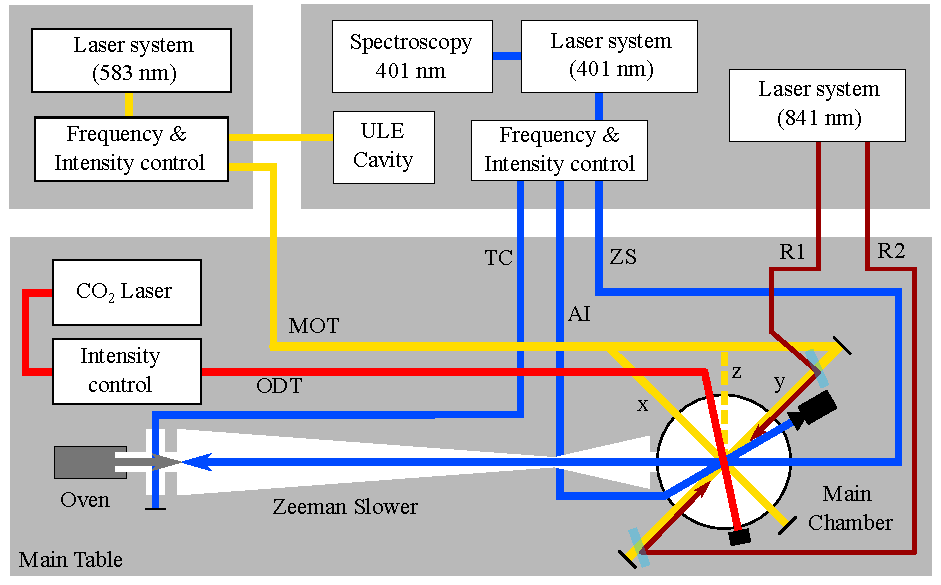
\includegraphics[width=1.\columnwidth]{table_set_up.pdf}
	\caption[Scheme of the experimental setup]{Scheme of the experimental setup. It is divided in three optical tables represented by gray areas. The 401nm laser system is used for the \acf{tc}, \acf{zs} and \acf{ai}. It is generated by a frequency doubled diode laser locked to a spectroscopic signal of the 401nm transition of $^{\text{168}}\text{Er}$. The 583nm laser system is used for the \acf{mot} and is frequency looked to an \acf{ule}. This trap uses 401nm laser beam in three spacial dimensions x, y and z. The $\text{CO}_{2}$ laser is used as main source of an \acf{odt}. The 841nm laser system is used to form the two lattice beams used for the Bragg Scattering process which will be described in next Chapter.}\label{fig:table_set_up}. 
\end{figure}

Most of the laser systems in this experiment produce resonant light for the $^{\text{168}}\text{Er}$ atomic transitions. For this reason, these light sources are kept on different optical tables separated from the \ac{uhv} system. Thus, unwanted atom-light interaction that could damage the cooling capabilities of the experiment is reduced. This laser light is guided into the main table by using optical fibers that can be blocked and unblocked through the use of \acp{aom} before the fiber coupler. Allowing for a fast response time (typically a few microseconds) and better control of the experimental phases.





%%% Local Variables: 
%%% mode: latex
%%% TeX-master: "Thesis"
%%% End: 